% ********** Chapter 1 **********
\chapter{JBoss und PHP}
\label{sec:chap2}

Die urspr"ungliche Planung sah vor diesem Teil der Aufgabe, der Integration von Turpitude in einen
J2EE-Application-Server und der Umsetzung der verschiedenen Enterprise Java Bean-Typen in PHP, einen
erheblichen Teil der zur Verf"ugung stehenden Zeit zu widmen. Wie allerdings in Kapitel \ref{sec:chap1:fazit}
beschrieben verschoben sich diese Priorit"aten im Laufe der Implementierung des ersten Teils der Aufgabenstellung,
wodurch erheblich weniger Zeit f"ur dieses Kapitel zur Verf"ugung stand. Nichtsdestotrotz soll an dieser Stelle
eine M"ogliche Anwendung f"ur Turpitude erarbeitet werden, um einen kleinen Teil der M"oglichkeiten die diese 
Bibliothek bietet aufzuzeigen. Weiterhin soll durch das Entwickeln einer solchen Beispielanwendung die
Einsatzf"ahigkeit Turpitudes unter m"oglichst realen Bedingungen nachgewiesen werden, und
eventuelle Fehler in der Bibliothek sollen auf diese Weise gefunden und behoben werden.

\section{Aufgabe}
\label{sec:chap2:task}

Ziel ist es eine M"oglichkeit zu schaffen die verschiedenen Enterprise Java Bean Typen mit 
PHP zu implementieren. Hierzu muss zuerst ein Weg gefunden werden der JVM, die den Application-Server 
ausf"uhrt die n"otigen Parameter zu "ubergeben die das Laden von Turpitude zur Laufzeit erm"oglichen.
W"unschenswert hierbei w"are, dass die n"otigen Bibliotheken nur einmal beim Start des Application-Servers
geladen werden, anstatt jeder installierten Anwendung mitgegeben werden zu m"ussen. Weiterhin muss gew"ahrleistet
werden dass Fehler in der geladenen nativen Bibliothek und in PHP auftretende Fehler m"oglichst nicht zum Absturz des
Application-Servers f"uhren. Ein weiteres wichtiges Ziel ist die Entwicklung eines Buildsystems das dem
Entwickler das unn"otige Schreiben von sogenanntem "'Boilerplate-Code"', Quelltext also der f"ur jede
Applikation immer gleich ist, abnimmt, der PHP-Entwickler der EJBs schreiben will soll nach M"oglichkeit
keinerlei Java-Quelltext schreiben m"ussen.


\section{EJB 3.0}
\label{sec:chap2:ejb3}

Obwohl innerhalb der Firma - im Gegensatz zu EJB 2.0 - nur sehr wenig Erfahrung mit der Enterprise Java Bean Specification in der
neuesten Version 3.0 (siehe \cite{EJBHP}) vorhanden war, wurde beschlossen das Projekt unter Einsatz dieser durchzuf"uhren. 
Diese Entscheidung fiel nicht nur um Erfahrungen mit dieser neuen Technologie zu sammeln, sondern auch um das Projekt zukunftssicherer 
zu machen.
Aus diesem Grund sollem an dieser Stelle kurz die Unterschiede zwischen EJB 2.0 und 3.0 umrissen werden, es wird dabei
davon ausgegangen, dass der Leser mit den Programmierkonzepten von EJB 2.0 zumindest im Groben vertraut ist.

Die fr"uheren J2EE 1.4 and EJB 2.1 Spezifikationen sind sehr komplex, Entwickler mussten sich mit dem EJB-Komponentenmodell,
verschiedenen APIs und Entwurfsmustern sowie XML Metainformationsdateien vertraut machen bevor sie auch nur anfangen konnten
benutzbare Softwaresysteme zu entwickeln. Diese Komplexit"at verhinderte nicht nur die schnelle Adaption von J2EE,
sondern f"uhrte auch dazu dass J2EE oft falsch eingesetzt wurde, was wiederum schlechtere anstatt bessere Software zur Folge hatte.
Man erkannte dass das urspr"unglich vorrangige Ziel von EJB - die Gew"ahrleistung transaktioneller Integrit"at "uber verteilte 
Applikationen hinweg - von "'Enterprise Applications"' gar nicht ben"otigt wurde.
Die EJB 3.0 Spezifikation versucht nun sich diesem Komplexit"atsproblem anzunehmen, und aus den Erfahrungen lange eingesetzter
und erfolgreicher Opensource Projekte wie beispielsweise \emph{Hibernate}
\footnote{Hibernate ist ein O/R Mapper, eine Middleware die das Abbilden von relationen Datenbanken auf objektorierte
Datenstrukturen erlaubt, siehe \cite{HIBERNATEHP}}
und \emph{XDoclet}
\footnote{XDoclet erm"oglicht das attributorientierte Arbeiten in Java-Versionen vor 5, indem es die annotierten Attribute
vor dem eigentlichen "ubersetzen mittels eines Pr"aprozessors in Java-Quelltext umwandelt, siehe \cite{XDOCLETHP}}
zu lernen. Sie basiert auf Java-Annotationen und POJOs
\footnote{POJO steht f"ur "'Plain Old Java Object"' und bedeutet "'ganz normales Java-Objekt"'. Insbesondere unterscheiden sie sich
von mit vielf"altigen externen Abh"angigkeiten belasteten Objekttypen.}
, und ist sehr viel leichter zu Verstehen als fr"uhere Versionen, ohne jedoch an M"achtigkeit einzub"ussen.

Mit Java Annotationen (siehe \cite{JAVAANNOTATIONS}) wurde Java erstmals in der Version 5 mit der M"oglichkeit ausgestattet 
den Quelltext mit Metadaten zu versehen.
Durch die Verwendung von Annotationen wird in EJB 3.0 zum einen die Anzahl von ben"otigten Klassen und Interfaces reduziert,
und zum anderen werden so Deployment Deskriptoren weitestgehend unn"otig, da f"ur Konfigurationsparameter nun sinnvolle Wertebelegungen
angenommen werden, und davon abweichende Werte durch Annotationen direkt im Quelltext der Java-Klassen untergebracht werden.
Weiterhin werden Annotationen verwendet um Abh"angigkeiten zur Umgebung und JNDI-Zugriffe zu spezifizieren und durch
Dependecy Injection
\footnote{Entwurfsmuster das dazu dient in einem objektorientierten System Abh"angigkeiten zwischen Komponenten oder Objekten 
zu minimieren, siehe \cite{DEPINJ}}
automatisch aufzul"osen.
Ausserdem wurde die Notwendigkeit abgeschafft von EJB-spezifischen Interfaces zu erben oder diese zu implementieren, Session Beans
ben"otigen kein Home-Interface mehr, Entity Beans sind nun einfach Java-Klassen (POJOs), um Persistenzeigenschaften zu realisieren
verwendet man die neue \emph{Java Persistence Architecture}, welche bessere M"oglichkeiten zur Abfrage, f"ur Mengenoperationen und
Vererbung bietet. Die Implementierung von in fr"uheren Standards vorgeschriebenen Lebenszyklus-Callbackmethoden ist jetzt optional.
Ein weiteres Merkmal von EJB 3.0 sind die sogenannten "'Interceptors"'. Hierbei handelt es sich um Methoden oder Klassen die mittels
Annotationen an Session- und Message Driven Beans und an deren Methoden angeh"angt werden k"onnen. Sobald das annotierte Element 
(englisch "'target"') aufgerufen wird ruft der Application Server automatisch den angeh"angten Interceptor auf.




\section{Infrastruktur}
\label{sec:chap2:infra}

Bevor mit der Bearbeitung der Aufgabe begonnen werden konnte musste zun"achst die n"otige Infrastruktur
geschaffen werden, allem voran die Auswahl des zu verwendenden Application Servers. Diese Wahl war leicht
zu treffen, der bei 1\&1 ausschlie\ss lich eingesetzten Application Server ist JBoss \cite{JBOSSHP}.
Folglich wurde ein JBoss in der Version 4.0.5 installiert, wobei darauf zu achten war dass der
nicht standardm"a\ss ig mitinstallierte Deployer f"ur EJB 3.0 Applikationen zus"atzlich ausgew"ahlt wurde.
Direkt nach der Installation konnte der Application Server problemlos gestartet werden.

Nun wurde f"ur das Projekt eine Verzeichnisstruktur aufgebaut wie Sun sie f"ur EJB-Projekte vorschl"agt, mit
eigenen Unterverzeichnissen f"ur die Quelltexte (src/), ben"otigte Bibliotheken (lib/), zus"atzliche 
Deploymentdeskriptoren (dd/) und die beim Buildprozess erzeugten Dateien (build/).
Da es sich um ein reines Java-Projekt handelte wurde als Buildsystem Apache Ant \cite{ANTHP} und nicht
wie f"ur Turpitude selbst Make gew"ahlt. Ant benutzt die XML-Datei "'build.xml"' wie make das "'Makefile"'
benutzt, dessen Wurzelknoten "'project"' heissen muss. Darunter werden die einzelnen Targets angelegt, die
wiederum anderen Targets als Abh"angigkeiten haben k"onnen. Als Name f"ur das Projekt wurde "'phpejb"' gew"ahlt,
die ben"otigten Klassen liegen im Package \emph{net.xp\_framework.phpejb}. Bevor mit der Programmierung
begonnen werden konnte mussten jedoch Targets f"ur das "Ubersetzen, Packen und Deployen der Anwendung angelegt,
sowie am Anfang der build.xml einige Konfigurationsparameter gesetzt werden.
Das "Ubersetzen geschieht im Target \emph{compile} und bereitete keine Schwierigkeiten. Die so erzeugten
.class-Dateien werden im Target \emph{package-ejb} in ein JAR gepackt, das den Namen \emph{phpejb.ejb3} tr"agt,
damit der JBoss erkennen kann welchen Deploy-Mechanismus er verwenden muss. Dieses JAR wird zusammen mit 
dem Deploymentdeskriptor \emph{application.xml} - in dem lediglich beschrieben wird welche Module enthalten sind - zu
dem \emph{Enterprise Archive} \emph{phpejb.ear} zusammengepackt, dies geschieht im Target \emph{assemble-app}.
Ein weiteres Target namens \emph{deploy} kopiert dieses in das Verzeichnis in dem der JBoss die auszubringenden
Applikationen erwartet. Schlussendlich wurde noch das Target \emph{clean}, das die w"ahrend des
Buildprozess erzeugten Dateien l"oscht, sowie das Target \emph{all} angelegt, welches als erstes Target in der
build.xml steht und deswegen ausgef"uhrt wird wenn Ant ohne Parameter aufgerufen wird, und die n"otigen Schritte
enth"alt die zur Erzeugung der \emph{phpejb.ear} n"otig sind. Somit waren die Grundlagen f"ur die weitere
Entwicklung gelegt, und es konnte ein zwar leeres, aber dennoch valides .ear erzeugt werden.

\subsection{Beispielanwendung}
\label{sec:chap2:infra:example}

Um erste Erfahrungen mit einer EJB 3.0 Anwendung zu sammeln sollte nun ein einfacher Service entwickelt werden.
Damit diese Arbeit auch sp"ater von Nutzen ist wurde beschlossen einen Service zu schreiben der das Verhalten
der in \ref{sec:chap1:impl} vorgestellten Anwendung \emph{EngineList} nachempfindet, und eine Liste der zur Verf"ugung 
stehenden JSR 223 Implementierungen zur"uckgibt.

Zu jedem EJB Service geh"ort ein beschreibendes Interface, das Interface f"ur diesen Service ist denkbar einfach,
enth"alt es doch nur eine Methode, \emph{getList()}. Durch die Annotation \emph{@Remote} wird angegeben, dass dieses
Interface auch von remote aufgerufen werden kann.
\begin{lstlisting}[caption=Testservice Interface]
@Remote
public interface EngineList {
    public List<String> getList();
}
\end{lstlisting}
Zu diesem Interface musste nun eine implementierende Klasse geschrieben werden, da der Service von remote aufgerufen
werden soll muss keine lokale Implementierung vorhanden sein, ein Remote-Bean kann sowohl lokal als auch remote
aufgerufen werden. Die simpelste EJB ist die Stateless Session Bean, und die Annotation \emph{@Stateless} gibt an
dass es sich bei dieser Bean um eine solche handelt.
\begin{lstlisting}[caption=Testservice Bean]
@Stateless
public class EngineListBean implements EngineList {
    public List<String> getList() {
    ...
    }
}
\end{lstlisting}
Die einfachste Methode einen EJB-Service zu testen ist einen Client zu schreiben, der in einer anderen JVM
ausgef"uhrt wird als der Application-Server, ein solcher Test zeigt nicht nur ob der Service funktioniert,
sondern auch ob das Deployment funktioniert hat, und der Service von aussen "uber JNDI aufgefunden und angesprochen
werden kann. Ein solcher JNDI-Lookup geschieht immer "uber einen Kontext, welcher die n"otigen Service-Provider
kennt. Der Lookup resultiert in einem Stub-Objekt, welches Aufrufe "uber die Netzverbindung an den Application-Server
weiterleitet.
\begin{lstlisting}[caption=Testservice Client]
InitialContext ctx = new InitialContext(env);
EngineList list = 
    (EngineList)ctx.lookup("phpejb/EngineListBean/remote");
List<String> lst = list.getList();
\end{lstlisting}
Der Aufruf ergab als einzige innerhalb des JBoss verf"ugbare JSR 223 Implementierung die standardm"a\ss ig in Java 6
enthaltene Javascript Engine Rhino von Mozilla. Nun mussten der den JBoss ausf"uhrenden JVM die n"otigen Parameter
mitgegeben werden, damit Turpitude innerhalb des Application Servers verf"ugbar wird (siehe auch \ref{sec:app1:exec}). 
Hierzu wurde ein Shell-Skript geschrieben, das die ben"otigten Umgebungsvariablen (LD\_LIBRARY\_PATH, JAVA\_HOME) setzt, 
und dann das eigentliche JBoss-Startskript \emph{run.sh} mit den n"otigen Parametern ausf"uhrt. 
Als dies getan war erschien Turpitude in der Liste der verf"ugbaren ScriptEngines, und es konnte mit der eigenlichen
Aufgabe begonnen werden.
\begin{lstlisting}[caption=JBoss Startskript]
#!/bin/sh
TURP_HOME=<PFAD>
PHP_HOME=<PFAD>
export JBOSS_HOME=/home/nsn/jboss-4.0.5.GA
export JAVA_HOME=/home/nsn/jdk1.6.0
export LD_LIBRARY_PATH=$LD_LIBRARY_PATH:$PHP_HOME/libs:$TURP_HOME
./run.sh --classpath=$TURP_HOME/turpitude.jar
\end{lstlisting}



\section{Stateless Session Beans}
\label{sec:chap2:slsb}

Die simpelste EJB ist die Stateless Session Bean, weswegen sie als erstes umgesetzt werden sollte.
Stateless Session Beans haben - wie der Name bereits vermuten l"a\ss t keinen eigenen Zustand, sie
k"onnen also keine Informationen "uber mehrere Anfragen hinweg vorhalten.

\subsection{Interface}
\label{sec:chap2:slsb:if}
Wie f"ur jede EJB muss auch f"ur die Stateless Session Bean zun"achst ein Interface definiert werden.
Das Interface f"ur diese Beispielanwendung ist denkbar einfach, es besteht lediglich aus einer einzigen
Methode, welche einen Namen als String entgegennimmt und einen String zur"uckgibt, der eine
Grussbotschaft enth"alt. 
\begin{lstlisting}[caption=Stateless Hello World Interface]
public interface SLHelloWorld {
    public String sayHello(String s);
}
\end{lstlisting}

\subsection{PHP-Implementation}
\label{sec:chap2:slsb:impl}

Die Implementation des Bean-Interfaces besteht aus zwei Teilen, zum einen dem Java-Teil, der die
ScriptEngine instantiiert, den PHP-Quelltext laedt und "ubersetzt und die entsprechenden PHP-Funktionen
aufruft, und zum anderen den PHP-Teil, der die eigentliche Interface-Implementierung enth"alt.
\begin{lstlisting}[caption=Java-Teil]
public String sayHello(String s) {
...
    ScriptEngineManager mgr = new ScriptEngineManager();
    ScriptEngine eng = mgr.getEngineByName("turpitude");
    Compilable comp = (Compilable)eng;
    CompiledScript script = comp.compile(/* Source */);
    Invocable inv = (Invocable)script;
    SLHelloWorld hw = 
        inv.getInterface(SLHelloWorld.class);
...
    return hw.sayHello(s);
}
\end{lstlisting}
Nat"urlich bietet Turpitude viele M"oglichkeiten die n"otige Funktionalit"at zu implementieren,
trotzdem wurde die vielleicht komplizierteste Variante gew"ahlt: das Implementieren des EJB-Interfaces in
PHP und das Aufrufen der PHP-Methoden "uber das \emph{javax.script.Invocable} Interface. Diese Entscheidung 
wurde vor allem vor dem Hintergrund getroffen, dass die Entwicklung einer PHP-Implementation eines Java-Interfaces
intuitiver erscheint, als das Entwickeln von PHP-Skripten die sich an eine nicht trivial ersichtliche
Konvention halten m"ussen um vom Java-Teil aufgerufen werden zu k"onnen. Ausserdem ist so ein 
generischer Adapter denkbar der beliebige Java-Interfaces auf passende PHP-Implementationen adaptiert,
oder zumindest ein Automatismus, der aus einem gegebenen Java-Interface und einer PHP-Implementierung den 
n"otigen Java-Quelltext automatisch erzeugt.
\begin{lstlisting}[caption=PHP-Implementierung]
<?php
class SLHelloWorld {
  function sayHello($s) {
    return 'The PHP-implementation says hello to '.$s;
  }
}
?>
\end{lstlisting}
Der Aufruf des SLHelloWorld-Service unterscheidet sich nicht von dem Aufruf des EngineList-Services, siehe \ref{sec:chap2:infra:example}.


\section{Stateful Session Beans}
\label{sec:chap2:sfsb}

Eine Stateful Session Bean ist ein EJB das seinen internen Status "uber mehrere Aufrufe hinweg beibehalten kann.
Methodenaufrufe des Client an einem bestimmten Stub werden immer an die selbe Bean-Instanz weitergeleitet, somit
behalten alle Felder der Bean ihre Werte solange der Client den Stub h"alt.
\begin{floatingfigure}[!h]{80mm}
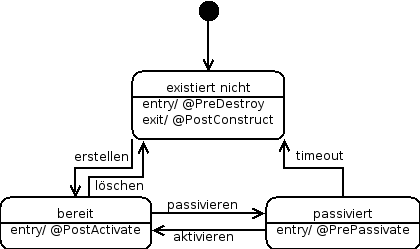
\includegraphics[width=75mm]{chap2/img/sfsbstates.png}
\caption{Lebenszyklus einer Stateful Session Bean, mit Annotationen}
\label{fig:sfsbstates}
\end{floatingfigure}
Zwar geschieht das Erstellen, Vorhalten und L"oschen der einzelnen Bean-Instanzen vollautomatisch durch den EJB-Container, 
trotzdem besteht manchmal die Notwendigkeit den Lebenszyklus einer Bean zu beeinflussen. Hierf"ur mussten in fr"uheren
EJB-Versionen sogenannte "'Lifecycle-Callbacks"' implementiert werden. In EJB 3.0 sind diese Callbacks "uberfl"ussig,
und werden durch spezielle Annotationen ersetzt, die zu bestimmten Zeitpunkten im Lebenszyklus aufzurufende Methoden
vermerken. Abbildung \ref{fig:sfsbstates} stellt den Lebenszyklus einer Stateful Session Bean zusammen mit den jeweiligen
Annotationen dar.
Die meisten dieser Annotationen sind sowohl f"ur Stateful, als auch f"ur Stateless Session Beans zul"assig,
im folgenden sollen die wichtigsten aufgef"uhrt werden:
\begin{description}
\item[@PostConstruct]
Die annotierte Methode wird direkt nachdem die Instanz erstellt wurde vom Container aufgerufen, @PostConstruct ist sowohl
f"ur Stateful als auch f"ur Stateless Session Beans zul"assig.
\item[@PreDestroy]
Die annotierte Methode wird aufgerufen bevor der Container eine unbenutzte oder ausgelaufene Instanz aus seinem Objektpool
l"oscht, @PreDestroy ist sowohl f"ur Stateful als auch f"ur Stateless Session Beans zul"assig.
\item[@PrePassivate]
Wenn eine Stateful Session Beans Instanz zu lange nicht aufgerufen wird kann der Container diese passivieren, und ihren
Zustand in seinem Cache zwischenspeichern. Eine mit @PrePassivate annotierte Methode wird direkt vor dem Passivieren aufgerufen.
\item[@PostActivate]
Wenn eine Anfrage an eine passivierte Bean gestellt wird wird eine neue Instanz der Bean-Klasse erzeugt und der vormalige
Zustand wieder hergestellt. Nachdem dies geschehen ist, aber bevor der Aufruf schliesslich an die Bean-Instanz weitergeleitet
wird wird die mit @PostActivate annotierte Methode aufgerufen. Diese Annotation ist nur f"ur Stateful Session Beans zul"assig.
\item[@Init]
Diese Annotation bezeichnet Initialisierungsmethoden f"ur eine Stateful Session Beans. Der Unterschied zu @PostConstruct
besteht darin, dass innerhalb einer Bean-Klasse mehrere Methoden mit @Init annotiert werden k"onnen, allerdings wird immer nur
eine dieser Methoden tats"achlich vom Container aufgerufen. Welche das ist bestimmt sich aus der Art und Weise, wie die
Bean erstellt wurde, n"aheres ist der EJB 3.0 \cite{EJBHP} zu entnehmen. Die @Init-Methode wird noch vor der 
@PostConstruct-Methode aufgerufen.
\end{description}


\subsection{Interface}
\label{sec:chap2:sfsb:if}

Um die zustandsvorhaltenden Eigenschaften der Stateful Session Bean zu testen enth"alt das Service-Interface eine Methode 
um den Namen der zu gr"u\ss enden Person zu setzen. Die Gru\ss methode selbst nimmt folglich keine Parameter entgegen, sondern
nutzt den zuvor gesetzten Namen um die Gru\ss botschaft zu erstellen.
\begin{lstlisting}[caption=Stateful Hello World Interface]
public interface SFHelloWorld {
    public void setName(String s) throws ScriptException;
    public String sayHello() throws ScriptException;
}
\end{lstlisting}

\subsection{PHP-Implementation}
\label{sec:chap2:sfsb:impl}

Im Gegensatz zum Service-Interface unterscheidet sich die Implementierung der Stateful Session Bean erheblich von der
Stateless Session Bean. Da der Zustand der Bean nicht im Java-Teil, sondern vom PHP-Code vorgehalten werden sollte
mussten Lebenszyklus-Methoden implementiert werden.

Zun"achst wurde die mit \emph{@PostConstruct} annotierte Methode \emph{initialize()} geschrieben, in der der Quelltext
"ubersetzt und eine Instanz der implementierenden PHP-Klasse erzeugt wird. Dieses Erzeugen geschieht mittels einer
Art "'friend-Methode"', aber es sind auch beliebige andere Methoden denkbar.
Sowohl das "ubersetzte Skript als auch das PHPObject der PHP-Klasse werden als Attribute der Bean gespeichert. 
Allerdings konnten diese Attribute aus zwei
Gr"unden nicht zur Speicherung des Zustandes genutzt werden: zum einen sollte im Hinblick auf eine m"ogliche
Automatisierung s"amtliche Funktionalit"at in PHP realisiert werden, und zum anderen kann innerhalb des Bean-Containers
nicht davon ausgegangen werden, dass die in ByteBuffern gespeicherten Informationen - der Zend-Opcode des "ubersetzten
Skriptes und vor allem der C-Pointer auf den Zval des PHP-Objektes - beim n"achsten Aufruf einer Bean-Methode noch valide 
sind. Folglich mussten der Bean zwei weitere Methoden hinzugef"ugt werden, die mit \emph{@PrePassivate} annotierte Methode
\emph{sleep()}, und die mit \emph{@PostActivate} annotierte Methode \emph{wakeUp()}. Als Methode zur Persistierung des
PHP-Objektes wurde der PHP-Mechanismus zur Serialisierung von Daten gew"ahlt, hierzu wurden der PHP-Klasse die Methoden
\emph{ser()} und \emph{unser()} hinzugef"ugt, erstere gibt einen String zur"uck der eine serialisierte Fassung des Objektes
enth"alt, letztere nimmt einen solchen String entgegen und stellt daraus den urspr"unglichen Zustand wieder her.
Damit gew"ahrleistet ist dass die oben angesprochenen Attribute der Java-Klasse nicht versehentlich persistiert werden 
werden die Referenzen der beiden Objekte auf null gesetzt.
Die Aufrufe der eigentlichen Service-Methoden werden genau wie bei der Stateless Session Bean mittels des Invocable-Interfaces
durchgef"uhrt, ihr Implementation in PHP gestaltete sich als trivial
\begin{lstlisting}[caption=PHP-Implementierung]
<?php
class SFHelloWorld {
  var $name = 'initial value';
  function setName($n) {
    $this->name = $n;
  }
  function sayHello() {
    return 'Stateful PHP says hello to '.$this->name;
  }
  function ser($obj) {
    return serialize($obj);
  }
  function unser($str) {
    $cpy = unserialize($str);
    $this->setName($cpy->name);
  }
}
\end{lstlisting}



\section{"Anderungen an Turpitude}
\label{sec:chap2:turp}

Im Laufe der Entwicklung dieser Beispielanwendungen zeigten sich einige Schwachstellen in
Turpitude, die aber behoben werden konnten. Die meisten aufgetretenen Probleme r"uhrten daher,
dass innerhalb eines J2EE Application Servers besondere Bedingungen vorherrschen.
Dieser Abschnitt soll diese Probleme und ihre Behebung erl"autern.

\subsection{finalize}
\label{sec:chap2:turp:final}

Eine Besonderheit f"ur eine Klasse wenn sie innerhalb eines Application Servers aufgerufen wird
ist, dass keine Garantie "uber die Lebenszeit und -Zyklen der Instanzen gegeben wird, ein Objekt kann
- immer entsprechend der J2EE-Spezifikation - mehrfach oder auch nur einfach benutzt werden, und
es besteht keine Kontrolle "uber die Laufzeit der ausf"uhrenden JVM.
Deswegen reichte der in der PHPScriptEngine eingebaut \emph{VMShutdown-Hook} nicht mehr aus um
den PHP-Interpreter aus dem Speicher zu entfernen und auf C-Ebene belegte Resourcen wieder
freizugeben. Java kennt zwar keine Destruktoren, aber jede Klasse erbt von \emph{Object} die
Methode \emph{finalize}, die jedesmal aufgerufen wird wenn das Objekt von der \emph{Garbage Collection}
aufger"aumt wird. 
Beim "uberschreiben dieser Methode ist es angebracht einen \emph{try-catch-finally}-Block
um die ausgef"uhrten Zeilen zu legen, und im finally-Teil \emph{super.finalize()} aufzurufen.
Jede in \emph{finalize} auftretende Exception unterbricht zwar das aufr"aumen, wird ansonsten
aber ignoriert.
Folglich wurde in der PHPScriptEngine die Methode finalize "uberschrieben, und innerhalb dieser
Methode wird \emph{shutDown} aufgerufen.

\subsection{Mehrfachinstanziierung}
\label{sec:chap2:turp:multi}

Wird innerhalb eines Java-Threads der PHP-Interpreter mehrfach instanziiert kann es zu Problemen
kommen: zum einen kann nicht mehr gew"ahrleistet werden dass die Ausf"uhrung des "ubersetzten
PHP-Quelltextes Fehlerfrei abl"auft, da unter Umst"anden w"ahrend der Ausf"uhrung die sogenannten
\emph{Executor Globals} (Skriptvariablen, Aufrufstacks und die Zend-Opcodes selbst) ver"andert werden,
und zum anderen kann der mehrfache Aufruf der \emph{startUp()}-Methode, in der der PHP-Interpreter
initialisiert wird, zu schweren Fehlern bis hin zu Abst"urzen der JVM f"uhren. Um dies zu verhindern
wurde die PHPScriptEngineFactory derart angepasst, dass sie eine abge"anderte Version Singleton-Patterns
implementiert um zu verhindern dass mehrere PHPScriptEngines gleichzeitig existieren. 
Da der Konstruktor der PHPScriptEngine \emph{protected} ist kann angenommen werden dass die 
Methode \emph{getScriptEngine()} der PHPScriptEngineFactory die einzige Stelle ist, an der
ScriptEngine-Instanzen erzeugt werden. So wurde der Factory ein privates, statisches Attribut \emph{MyEngine} 
hinzugef"ugt, welches die Singleton-Instanz der PHPScriptEngine vorh"alt. Dieses Attribut ist zu Begin
\emph{NULL}, und wird beim ersten Aufruf von \emph{getScriptEngine()} gesetzt, jeder weitere Aufruf
dieser Methode gibt nur noch eine Referenz auf diese einzige ScriptEngine zur"uck. Das Erzeugen des
Singletons wird zus"atzlich durch einen \emph{synchronized}-Bl"ock vor gleichzeitiger
Mehrfachausf"uhrung gesch"utzt.
\begin{lstlisting}[caption=Singleton-Erzeugung]
public ScriptEngine getScriptEngine() {
    if (MyEngine == null) {
        synchronized (PHPScriptEngineFactory.class) {
            if (MyEngine == null)
                MyEngine = new PHPScriptEngine(this);
        }
    }
    return MyEngine;
}
\end{lstlisting}



% ********** Chapter 1 **********
\section{Fazit}
\label{sec:chap1:fazit}

Im Laufe dieses Kapitels wurde eine m"achtige Bibliothek entwickelt, die nicht nur das Ausf"uhren von
PHP-Skripten aus einer Java-Laufzeitumgebung heraus erm"oglicht, sondern viel weiter geht und die beiden
Programmiersprachen eng miteinander verbindet. Dem PHP-Entwickler wird die M"oglichkeit geboten den
vollen Funktionsumfang von Java inklusive aller verf"ugbaren Java-Bibliotheken zu nutzen, Objekte zu erzeugen,
auf deren Felder und Methoden zuzugreifen und diese auf intuitive und einfache Weise in PHP zu nutzen.
Der Java-Entwickler kann PHP-Skripte nicht nur ausf"uhren und ihnen Daten "ubergeben und von ihnen erzeugte
Daten zur"uckzuerhalten, er kann nicht nur gezielt Funktionen und Methoden innerhalb eines PHP-Skriptes
aufrufen, sondern er kann sogar Java-Interfaces direkt in PHP implementieren, oder bereits bestehende PHP-Klassen
in ein Java-Interface wrappen und transparent mit ihnen wie mit jedem anderen Java-Objekt umgehen.

Dieser Funktionsumfang macht Turpitude einzigartig. Es existieren zwar zwei "'Konkurrenzprodukte"' auf dem
Markt - die JSR223-Implementation von Zend und die PHP/Java-Bridge \cite{BRIDGEHP} - allerdings implementieren
beide weder den vollen Umfang des JSR223, noch halten sie die aktuelle Spezifikation ein. Weiterhin ist die
Zend-Implementation nicht Quelloffen, sprich es ist einem Anwender nicht m"oglich ein eigenes PHP in Java
zu benutzen, mit allen Extensions die er braucht, und es ist ebenfalls unm"oglich sie auf nicht explizit
unterst"utzten Plattformen einzusetzen. Die PHP/Java-Bridge ist zwar im Quelltext verf"ugbar, aber sie
benutzt eine TCP-Verbindung um mit einer laufenden Java-Umgebung zu kommunizieren. Diese Kommunikation
ist basiert ausserdem noch auf XML, die Nachteile einer solchen Kommunikation wurden in Kapitel \ref{sec:background}
hinl"anglich beschrieben. 

Somit wurden alle am Anfang des Kapitels gesteckten Ziele nicht nur erreicht sondern in vielen F"allen sogar
"ubererf"ullt.

Die Implementation der Bibliothek selbst wurde haupts"achlich durch zwei Faktoren erschwert:\\
Zum einen ist die JSR223-Spezifikation in vielen Detailfragen nur "au\ss erst ungenau und erscheint ausserdem
in einigen Bereichen etwas undurchdacht. Dies lies sich allerdings in den meisten F"allen durch eine
angemessene Portion Pragmatismus sehr schnell und zur Zufriedenheit Aller l"osen. Deutlich mehr Zeit
kostete die Mangelhafte Dokumentation der Zend-Engine. Viele Probleme konnten nur durch langwieriges
Ausprobieren und das Lesen des Zend-Quelltextes gel"ost werden, was oft zu unn"otigen Verz"ogerungen 
des Projektes f"uhrte. Abgesehen von den veralteten und nicht gepflegten Dokumentationsbruchst"ucken
auf der PHP-Seite \cite{PHPHP} war die einzig wirklich hilfreiche "'Dokumentation"' die, die durch das Programm
\emph{LXR} (siehe \cite{LXRHP}) erzeugt wird und unter \cite{PHPLXR} verf"ugbar ist. Der Quelltext
von PHP selbst stellt weitere Herausforderungen, so ist er nur sehr unzureichend kommentiert, und verwendet
einige eher "'interesante"' Konzepte. Das verdeutlichen am Besten einige Beispiele, zum einen die 
Implementierung einer verketteten Liste:
\begin{lstlisting}[caption=Verkettete Liste im Zend-Code]
typedef struct _zend_llist_element {
    struct _zend_llist_element *next;
    struct _zend_llist_element *prev;
    char data[1]; /* Needs to always be last in the struct */
} zend_llist_element;
...
zend_llist_element *le;
...
opline_ptr = (zend_op *)le->data;
\end{lstlisting}
Hier wird genau ein Byte Speicher reserviert, es werden allerdings Pointer an diese Stelle geschrieben,
die mindestens vier Bytes lang sind - ein Voidpointer w"are vielleicht passender gewesen.
Zum anderen noch ein Ausschnitt aus der de-serialisierungsroutine. Hier wurden zwar Kommentare
verwendet, allerdings zeugen sie an dieser Stelle nicht unbedingt von einer guten Organisation:
\begin{lstlisting}[caption=lustiges Beispiel f"ur Zend-Code]
yy13:   ++YYCURSOR;
    goto yy14;
yy14:
{
    /* this is the case where we have less data than planned */
    php_error_docref(
        NULL TSRMLS_CC, 
        E_NOTICE, 
        "Unexpected end of serialized data");
    return 0; /* not sure if it should be 0 or 1 here? */
}
\end{lstlisting}

Trotz dieser Probleme konnte ein benutzbares Softwaresystem erstellt werden, auch wenn Turpitude sicherlich
noch keinen Produktionsstatus erreicht hat, hierzu muss der Quelltext noch hinreichend auf Speicherlecks
"uberpr"uft werden, da der Einsatz in einem Web- oder Application-Server immer lange Laufzeiten mit sich bringt,
und Speicherlecks in diesen F"allen besonders gravierend sind. Weiterhin kann an vielen Stellen unn"otig gewordener
Quelltext entfernt oder "ahnliche Quelltextstellen zu eigenen Funktionen refaktoriert werden. Die Begrenzte Zeit
dieser Arbeit l"a\ss t solche "'Sch"onheitsoperationen"' aber leider nicht zu.

Nach Einsch"atzung des Autors kann Turpitude zu diesem Zeitpunkt aber schon guten Gewissens eingesetzt werden um 
nicht Unternehmenskritische Anwendungen zu entwickeln, vor allem weil eventuelle qualitative Verbesserungen
sich nicht mehr auf die Schnittstellen auswirken werden. Es gilt allerdings zu beachten dass die Bibliothek unter
keinen Umst"anden genutzt werden sollte um nicht-vertrauensw"urdige PHP-Skripte auszuf"uhren, zum einen weil
nicht alle Grenzf"alle ausgetestet wurden, und zum anderen weil durch den Zugriff auf Java-Klassen die PHP-eigenen
Schutzmechanismen ausgehebelt werden k"onnten. Ein solcher Einsatz beispielsweise um Kunden auf einem Java-Webserver 
PHP anzubieten w"are - zumindest zu diesem Zeitpunkt - grob fahrl"assig.

Im Laufe der Implementation wurde deutlich dass eine - im Gegensatz zur urspr"unglichen Planung - vollst"andige
Implementation des JSR223 und vor allem der Zugriff auf Java-Funktionalit"at aus dem PHP-Interpreter heraus
dem Unternehmen und der Abteilung viele Vorteile bringen w"urde, weswegen
deutlich mehr Zeit in die Entwicklung der Bibliothek investiert als eigentlich geplant. Dies f"uhrte nun
dazu dass f"ur den Rest der Aufgabe deutlich weniger Zeit zur Verf"ugung stand, weswegen in diesen Bereichen an
Umfang gek"urzt werden musste.

% ********** End of chapter **********





% ********** End of chapter **********
